%% !TEX program = xelatex
\documentclass[12pt,final]{novelette} % font size, twoside, twocolumn, draft-final, use extarticle for 8-20pt

\title{Calculus III Final 2541}
\author{Kaka Cring}
\date{\today}

\newcommand{\qmarki}[1]{\mbox{(#1 คะแนน)}}
\newcommand{\qmark}[1]{{%
      \unskip\nobreak\hfil\penalty50
      \hskip2em\hbox{}\nobreak\hfil\qmarki{#1}%
      \parfillskip=0pt \finalhyphendemerits=0 \par}}

\begin{document}

\thispagestyle{empty}
\vspace*{-6em}

\noindent
\fbox{
    \parbox[c][1.6em]{449pt}{\centering\bfseries
        ข้อสอบภาคต้น วิชา 2301217 Calculus III ปีการศึกษา 2541
    }
}

\bigskip

\begin{question}
    \item {}
    \begin{question}
        \item
        จากสมการพื้นผิว $x^2 + y^2 + z^2 + 2yz = 0$
        จงหา เมตริกซ์ของการเปลี่ยนทิศทางของแกนพิกัดที่ทำให้สมการใหม่ที่ได้อยู่ในรูป \
        $\lambda_1(x')^2 + \lambda_2(y')^2 + \lambda_3(z')^2 = k$ \\
        เมื่อเทียบกับพิกัดใหม่ $(X'Y'Z')$

        % ----------------------------------------
        \bigskip
        Let $
            A = \mqty[
                1 & 0 & 0 \\
                0 & 1 & 1 \\
                0 & 1 & 1 \\
            ]
        $.
        Then the equation is $
            \mqty[x & y & z]A\mqty[x \\ y \\ z] = 0
        $.\\[.5em]
        We find the eigenvalues of $A$.
        \begin{align*}
            \det(A - \lambda I)             & = 0                                                     \\
            \mqty|
            1 - \lambda                     & 0                                         & 0           \\
            0                               & 1 - \lambda                               & 1           \\
            0                               & 1                                         & 1 - \lambda \\
            |                               & = 0                                                     \\
            (1 - \lambda)^3 - (1 - \lambda) & = 0                                                     \\
            (1 - \lambda)^2 - 1             & = 0 \qquad \mathrm{or} \qquad \lambda = 1               \\
            1 - \lambda                     & = \pm 1                                                 \\
            \lambda                         & = 0, 2
        \end{align*}

        Let $\lambda_1 = 0, \lambda_2 = 1, \lambda_3 = 2$. \\
        Find the component vectors $v_1, v_2, v_3$ of the transformation matrix $P$.

        \medskip
        For $v_1$;
        \begin{align*}
            (A - \lambda_1 I) v_1     & = \mathbf{0}         \\
            \begin{bmatrix}
                1 & 0 & 0 \\
                0 & 1 & 1 \\
                0 & 1 & 1 \\
            \end{bmatrix}
            \begin{bmatrix}
                x \\ y \\ z
            \end{bmatrix}
                                      & = \begin{bmatrix}
                                              0 \\ 0 \\ 0
                                          \end{bmatrix}     \\
            \intertext{We get $x = 0$ and $y + z = 0$, therefore $y = -z$. Let $y = t$.}
            \lVert v_1 \rVert         & = 1                  \\
            \sqrt{0^2 + t^2 + (-t)^2} & = 1                  \\
            t                         & = \pm \frac1{\sqrt2}
        \end{align*}
        Choose $v_1 = \mqty[0 \\ \frac1{\sqrt2} \\ -\frac1{\sqrt2}]$.

        \medskip
        For $v_2$;
        \begin{align*}
            (A - \lambda_2 I)v_2 & = \mathbf{0}     \\
            \begin{bmatrix}
                0 & 0 & 0 \\
                0 & 0 & 1 \\
                0 & 1 & 0 \\
            \end{bmatrix}
            \begin{bmatrix}
                x \\ y \\ z
            \end{bmatrix}
                                 & = \begin{bmatrix}
                                         0 \\ 0 \\ 0
                                     \end{bmatrix}
        \end{align*}
        Since $\lVert v_2 \rVert = 1$, we get $x = \pm 1, y = 0, z = 0$.
        Choose $v_2 = \mqty[1 \\ 0 \\ 0]$.

        \medskip
        For $v_3$;
        \begin{align*}
            (A - \lambda_3 I)v_3 & = \mathbf{0}     \\
            \begin{bmatrix}
                -1 & 0  & 0  \\
                0  & -1 & 1  \\
                0  & 1  & -1 \\
            \end{bmatrix}
            \begin{bmatrix}
                x \\ y \\ z
            \end{bmatrix}
                                 & = \begin{bmatrix}
                                         0 \\ 0 \\ 0
                                     \end{bmatrix}
        \end{align*}
        We get $x = 0, y - z = 0$. Since $\lVert v_3 \rVert = 1$, we get $y = z = \pm \frac1{\sqrt2}$.
        Choose $v_3 = \mqty[0 \\ \frac1{\sqrt2} \\ \frac1{\sqrt2}]$.

        Therefore the transformation matrix is
        \begin{align*}
            P & = \begin{bmatrix}
                      v_1 & v_2 & v_3
                  \end{bmatrix}                             \\
              & = \boxed{\begin{bmatrix}
                                 0               & 1 & 0              \\
                                 \frac1{\sqrt2}  & 0 & \frac1{\sqrt2} \\
                                 -\frac1{\sqrt2} & 0 & \frac1{\sqrt2}
                             \end{bmatrix}}
        \end{align*}

        and the new equation is $(y')^2 + 2(z')^2 = 0$.

        % ----------------------------------------

        \item
        จงเขียนสมการใหม่ของสมการพื้นผิว $x^2 + y^2 + z^2 + 2yz + z - y = 0$
        พร้อมทั้งวาดภาพของพื้นผิวนี้ด้วย \qmark{14}

        % ----------------------------------------
        \bigskip
        Using the relation $X = PX'$ and the properties of orthogonal matrix, we transform the surface equation into
        \begin{align*}
            0(x')^2 + 1(y')^2 + 2(z')^2 +
            \begin{bmatrix}
                0 & -1 & 1
            \end{bmatrix}
            P
            \begin{bmatrix}
                x' \\ y' \\ z'
            \end{bmatrix}
                                                 & = 0  \\
            (y')^2 + 2(z')^2 +
            \begin{bmatrix}
                -\sqrt2 & 0 & 0
            \end{bmatrix}
            \begin{bmatrix}
                x' \\ y' \\ z'
            \end{bmatrix}
                                                 & = 0  \\
            \Aboxed{(y')^2 + 2(z')^2 - \sqrt2 x' & = 0}
        \end{align*}
        relative to new coordinate axes $X'Y'Z'$.

        This is an elliptic paraboloid that has generator along positive $X'$ axis.

        \begin{figure}[h]
            \centering
            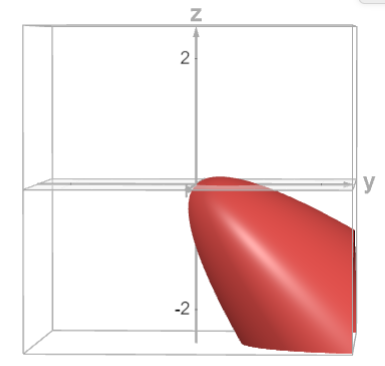
\includegraphics[scale=0.7]{images/Surface12.png}
        \end{figure}

        % ----------------------------------------
    \end{question}

    \item {}
    \begin{question}
        \item
        ให้ $C$ เป็นเส้นโค้ง กำหนดโดยสมการ
        $$
            \vec{r}(t) = \left(\frac{t^3}{3}, t^2, 2t\right), \quad t \in [0, 3]
        $$
        จงหาความยาวของเส้นโค้ง $C$ และความโค้งของเส้นโค้ง $C$ ณ จุด $\vec{r}(t)$ ใด ๆ \qmark{8}

        % ----------------------------------------
        \bigskip
        First, we find the first and second derivatives of $\vec{r}(t)$.
        \begin{align*}
            \vec{r}'(t)  & = \left(t^2, 2t, 2\right) \\
            \vec{r}''(t) & = \left(2t, 2, 0\right)
        \end{align*}
        The length can be written as an integral
        \begin{align*}
            L & = \int_C \dd{S}                             \\
              & = \int_0^3 \lVert \vec{r}'(t) \rVert \dd{t} \\
              & = \int_0^3 \sqrt{t^4 + 4t^2 + 4} \dd{t}     \\
              & = \int_0^3 |t^2 + 2| \dd{t}                 \\
              & = \left[ \frac{t^3}3 + 2t \right]_0^3       \\
              & = 15
        \end{align*}
        Therefore the length of $C$ is $\boxed{15\,\mathrm{units}}$.

        \medskip
        The curvature is given by the formula
        $$
            \kappa = \frac{\lVert \vec{r}'(t) \times \vec{r}''(t) \rVert}{\lVert \vec{r}'(t) \rVert^3}
        $$

        Find the cross product
        \begin{align*}
            \begin{bmatrix}
                t^2 \\ 2t \\ 2
            \end{bmatrix}
            \times
            \begin{bmatrix}
                2t \\ 2 \\ 0
            \end{bmatrix}
             & =
            \begin{bmatrix}
                -4 \\ 4t \\ -2t^2
            \end{bmatrix}
        \end{align*}

        The curvature is
        \begin{align*}
            \kappa & = \frac{\sqrt{(-4)^2 + (4t)^2 + (-2t^2)^2}}{\left(\sqrt{(t^2)^2 + (2t)^2 + 2^2}\right)^3} \\
                   & = \frac{2\sqrt{4+4t^2+t^4}}{\left(t^4 + 4t^2 + 4\right)^{3/2}}                            \\
                   & = \boxed{\frac{2}{t^4 + 4t^2 + 4}}
        \end{align*}
        % ----------------------------------------

        \item
        ให้ $C$ เป็นเส้นโค้ง กำหนดโดยสมการ
        $$
            \vec{r}(t) = \left(\frac23 t^3, \frac{t^2}{2}, 2t\right), \qquad t \in [0, 3]
        $$
        จงหาเวกเตอร์หนึ่งหน่วยสัมผัส เวกเตอร์นอร์มัลหลัก และเวกเตอร์นอร์มัลคู่ ณ จุด $\vec{r}(1)$ \qmark{8}

        % ----------------------------------------
        \bigskip
        The unit tangent vector is
        \begin{align*}
            \vec{T}(t) & = \frac{\vec{r}'(t)}{\lVert \vec{r}'(t) \rVert}    \\
                       & = \frac{(2t^2, t, 2)}{\sqrt{(2t^2)^2 + t^2 + 2^2}} \\
            \vec{T}(1) & = \frac{(2, 1, 2)}{\sqrt{4 + 1 + 4}}               \\
                       & = \boxed{\left(\frac23, \frac13, \frac23\right)}
        \end{align*}

        We need the derivative of the unit tangent vector to find normal vector. Let $\vec{u} = (2t^2, t, 2)$.
        \begin{align*}
            \vec{T}'(t) & = \frac{\vec{u}'\lVert \vec{u} \rVert^2 - \vec{u} (\vec{u} \cdot \vec{u}')}{\lVert \vec{u} \rVert^3} \\
                        & = \frac{(4t, 1, 0)(4t^4 + t^2 + 4) - (2t^2, t, 2)(8t^3 + t)}{(4t^4 + t^2 + 4)^{3/2}}                 \\
            \vec{T}'(1) & = \frac{9(4, 1, 0) - 9(2, 1, 2)}{27}                                                                 \\
                        & = \left(\frac23, 0, -\frac23\right)
        \end{align*}

        The principal normal vector is
        \begin{align*}
            \vec{N}(t)  & = \frac{\vec{T}'(t)}{\lVert \vec{T}'(t) \rVert}               \\
            \vec{N}'(1) & = \frac{3}{2\sqrt2} \left(\frac23, 0, -\frac23\right)         \\
                        & = \boxed{\left(\frac{1}{\sqrt2}, 0, -\frac{1}{\sqrt2}\right)}
        \end{align*}
        The binormal vector is
        \begin{align*}
            \vec{B}(t) & = \vec{T}(t) \times \vec{N}(t)                                                                      \\
                       & = \left(\frac23, \frac13, \frac23\right) \times \left(\frac{1}{\sqrt2}, 0, -\frac{1}{\sqrt2}\right) \\
                       & = \boxed{\frac{1}{3\sqrt2}\left(-1, 4, -1\right)}
        \end{align*}
        % ----------------------------------------
    \end{question}

    \item {}
    \begin{question}
        \item
        จงเขียน $\iiint_D xz^2 \dd{v}$ ในระบบพิกัดทรงกลม เมื่อ $D$ เป็นวัตถุทรงตัน ที่อยู่ภายในทรงกลม \\
        $x^2 + y^2 + (z-2)^2 = 4$
        และอยู่ภายนอกกรวย $\sqrt3 z = \sqrt{x^2 + y^2}$ \\
        (เขียนภาพโดเมนของการอินทิเกรตและไม่ต้องคำนวณค่า) \qmark{6}

        % ----------------------------------------
        \bigskip
        Change to spherical coordinate system

        Sphere;
        \begin{align*}
            (\rho \sin \phi)^2 + (\rho \cos \phi - 2)^2 & = 4           \\
            \rho^2 - 4 \rho \cos \phi + 4               & = 4           \\
            \rho                                        & = 4 \cos \phi
        \end{align*}

        Cone;
        \begin{align*}
            \sqrt3 \rho \cos \phi & = \rho \sin \phi \\
            \cot \phi             & = \frac1{\sqrt3} \\
            \phi                  & = \frac{\pi}{3}
        \end{align*}

        Therefore the integral is
        $$
            \int_0^{2\pi} \int_{\pi/3}^{\pi/2} \int_0^{4\cos\phi} \rho \sin\phi \cos\theta (\rho \cos\phi)^2 \rho^2 \sin\phi \dd{\rho} \dd{\phi} \dd{\theta}
        $$
        or simplified to
        $$
            \boxed{\int_0^{2\pi} \int_{\pi/3}^{\pi/2} \int_0^{4\cos\phi} \rho^5 \sin^2\phi \cos^2\phi \cos\theta \dd{\rho} \dd{\phi} \dd{\theta}}
        $$
        % ----------------------------------------

        \item
        ให้ $S$ เป็นทรงตันที่ปิดล้อมด้วยผิว $y = 4x^2 + 9z^2$, $z = x^2$, $z = 1$ และ $y = 0$ \\
        จงเขียน $\iiint_S f(x, y, z) \dd{v}$ โดยใช้อินทิกรัลซ้อน โดยมีลำดับการอินทิเกรต $\dd{y} \dd{z} \dd{x}$ \qmark{6}

        % ----------------------------------------
        \bigskip
        $$
            \boxed{\int_{-1}^1 \int_{x^2}^1 \int_0^{4x^2+9z^2} f(x, y, z) \dd{y} \dd{z} \dd{x}}
        $$
        % ----------------------------------------

        \item
        จงเขียนอินทิกรัล \quad $\displaystyle \int\limits_0^{\sqrt3} \int\limits_{-\sqrt{3-y^2}}^{\sqrt{3-y^2}} \int\limits_{x^2+y^2}^{2+\sqrt{4-x^2-y^2}} f(x, y, z) \dd{z}\dd{x}\dd{y}$ \\[.5em]
        ในระบบพิกัดทรงกระบอก \qmark{6}

        % ----------------------------------------
        \bigskip
        Find boundaries in cylindrical coordinate system
        $$ r^2 \leq z \leq 2 + \sqrt{4 - r^2} $$
        $$ -\sqrt{3-(r\sin\theta)^2} \leq r \cos\theta \leq \sqrt{3-(r\sin\theta)^2} \implies 0 \leq r \leq \sqrt3 $$
        $$ 0 \leq r \sin\theta \leq \sqrt3 \implies 0 \leq \sin\theta \leq 1 \implies 0 \leq \theta \leq \pi $$

        $$
            \boxed{\int_0^{\pi} \int_{0}^{\sqrt3} \int_{r^2}^{2+\sqrt{4-r^2}} f(x, y, z)\, r \dd{z} \dd{r} \dd{\theta}}
        $$
        % ----------------------------------------
    \end{question}

    \item {}
    จงเปลี่ยนอินทิกรัล $\displaystyle \int\limits_{-2}^2 \int\limits_{-\sqrt{4-x^2}}^0 \int\limits_0^{\sqrt{4-x^2-y^2}} z^2 \sqrt{x^2 + y^2 + z^2} \dd{z} \dd{y} \dd{x}$ \\[.5em]
    ให้อยู่ในระบบพิกัดทรงกลม พร้อมทั้งเขียนโดเมนของการอินทิเกรต และหาค่าอินทิกรัลด้วย \qmark{8}

    % ----------------------------------------
    \bigskip
    Find boundaries in spherical coordinate system
    $$ 0 \leq \rho \cos\phi \leq \sqrt{4 - (\rho \sin\phi)^2} \implies 0 \leq \rho \leq 2 \implies 0 \leq \phi \leq \frac{\pi}{2} $$
    $$ -\sqrt{4 - (\rho \sin\phi \cos\theta)^2} \leq \rho \sin\phi \sin\theta \leq 0 \land -2 \leq \rho \sin\phi \cos\theta \leq 2 \implies -\pi \leq \theta \leq 0$$

    \begin{align*}
        \int_{-\pi}^0 \int_0^{\pi/2} \int_0^2 (\rho \cos\phi)^2 \rho \rho^2 \sin\phi \dd{\rho} \dd{\phi} \dd{\theta}
         & = \int_0^2 \rho^5 \dd{\rho} \int_0^{\pi/2} \sin \phi \cos^2\phi \dd{\phi} \int_{-\pi}^0 \dd{\theta} \\
         & = \frac{2^6}{6} \left[-\frac{\cos^3\phi}{3}\right]_0^{\pi/2} \pi                                    \\
         & = \frac{32}{3} \frac{1}{3} \pi                                                                      \\
         & = \boxed{\frac{32\pi}{9}}
    \end{align*}
    % ----------------------------------------

    \item {}
    \begin{question}
        \item
        จงหาค่า $\int_C (x + y + z - 1) \dd{s}$ เมื่อ $C$ เป็นส่วนโค้ง $y = x^2, z + y = 1$ จากจุด $(0,0,1)$ ไปยังจุด $(1,1,0)$ \qmark{8}

        % ----------------------------------------
        \bigskip
        The path is given by vector
        $$
            \vec{r}(t) = (t, t^2, 1-t^2), \qquad t \in [0, 1]
        $$
        The integral is
        \begin{align*}
            \int_C (x + y + z - 1) \dd{s}
             & =\int_0^1 (t + 1 - 1) \lVert \vec{r}'(t) \rVert \dd{t}  \\
             & =\int_0^1 t \sqrt{1 + (2t)^2 + (-2t)^2} \dd{t}          \\
             & = \frac1{16} \left[\frac23 (1 + 8t^2)^{3/2} \right]_0^1 \\
             & = \frac1{24} (27 - 1)                                   \\
             & = \boxed{\frac{13}{12}}
        \end{align*}
        % ----------------------------------------

        \item
        จงหาค่า $\displaystyle \int_C \frac{x}{x^2+y^2+1} \dd{x} + \frac{y}{x^2+y^2+1} \dd{y}$ เมื่อ $y$ เป็นเส้นโค้ง
        กำหนดโดยสมการ \\[.5em]
        $\displaystyle \vec{r}(t) = (e^t \cos t, e^t), \quad 0 \leq t \leq \frac{\pi}{2}$ \qmark{8}

        % ----------------------------------------
        \bigskip
        Let $\displaystyle\vec{F}(x, y) = \left(\frac{x}{x^2+y^2+1}, \frac{y}{x^2+y^2+1}\right)$.

        \medskip
        $\vec{F}$ is a gradient function on the surface $\mathbb{R}^2 - \{(0,0)\}$
        since there exists
        $$\phi(x, y) = \frac12 \ln\left(x^2+y^2+1\right)$$
        such that $\nabla\phi = F$.

        \medskip
        By the fundamental theorem of calculus of line integral part ii, we get that
        \begin{align*}
            \int_C \vec{F} \cdot \dd{\vec{r}} & = \phi(B) - \phi(A)                                 \\
                                              & = \phi(0, e^{\pi/2}) - \phi(1, 1)                   \\
                                              & = \boxed{\frac12 \ln\left(\frac{1+e^\pi}{3}\right)}
        \end{align*}
        % ----------------------------------------
    \end{question}

    \item {}
    ให้ $C$ เป็นอาณาบริเวณที่ปิดล้อมด้วยเส้นโค้ง $y = x^3$ เส้นตรง $x + y = 2$ และ $x = 0$ ในทิศทางทวนเข็มนาฬิกา

    จงหา $\int_C \vec{F} \cdot \dd{\vec{r}}$ เมื่อ $\vec{F}(x, y) = (x^3y^2 + e^{x^2}, \tan y + e^y + yx^2)$ \qmark{8}

    % ----------------------------------------
    \bigskip
    Use Green's theorem; Let $\vec{F}(x, y) = (P(x, y), Q(x, y))$ and $R$ is the region bounded by $C$,
    \begin{align*}
        \int_C \vec{F} \cdot \dd{\vec{r}} & = \ointctrclockwise_C P \dd{x} + Q \dd{y}                              \\
                                          & = \iint_R \left(\pdv{Q}{x} - \pdv{P}{y}\right) \dd{A}                  \\
                                          & = \int_0^1 \int_{x^3}^{2-x} \left(2xy - 2x^3y\right) \dd{y} \dd{x}     \\
                                          & = \int_0^1 \left[(x - x^3)y^2\right]_{x^3}^{2-x} \dd{x}                \\
                                          & = \int_0^1 (x - x^3)((2-x)^2 - (x^3)^2) \dd{x}                         \\
                                          & = \int_0^1 (x - x^3)(4 - 4x + x^2 - x^6) \dd{x}                        \\
                                          & = \int_0^1 4x - 4x^2 + x^3 - x^7 - 4x^3 + 4x^4 - x^5 + x^9 \dd{x}      \\
                                          & = 2 - \frac43 + \frac14 - \frac18 - 1 + \frac45 - \frac16 + \frac1{10} \\
                                          & = \boxed{\frac{21}{40}}
    \end{align*}
    % ----------------------------------------

    \item {}
    จงหาค่าของ $\iint_S (1-x)yz \dd{s}$ โดยให้พื้นผิว $S$ เป็นส่วนหนึ่งของพื้นผิว $y^2 = 1-x$, $x \geq 0$ และ $0 \leq z \leq 3$ \qmark{8}

    % ----------------------------------------
    \bigskip
    Think of the region $S$ as if it was a collection of paths $\vec{r}(t) = (1-t^2, t, z), \quad t \in [-1, 1]$ on $XY$ plane and has constant values of $z$.
    Then the integral can be written as
    \begin{align*}
        \iint_S(1-x)yz \dd{s} & = \int_0^3 \int_{-1}^1 t^2 \cdot t z \lVert \vec{r}'(t) \rVert \dd{t} \dd{z} \\
                              & = \int_{-1}^1 t^3 \sqrt{4t^2+1} \dd{t} \int_0^3 z \dd{z}
    \end{align*}
    Since this is an odd function, the integral collapses to $\boxed{0}$.
    % ----------------------------------------

    \item {}
    กำหนดให้ $\vec{F}(x, y, z) = (y^2 + z^2 + 6zx, 2y(x + e^{y^2}) + 3y^2z, 2xz + y^3 + 3x^2)$

    \begin{question}
        \item
        จงหา $\int_C \vec{F} \cdot \dd{\vec{r}}$ เมื่อ $C$ เป็นเส้นโค้งที่มีสมการ
        $$
            \vec{r}(t) = (t \sin t, 3 \cos t, 2 \cos t - \sin t), \quad t \in \left[0, \frac\pi2\right]
        $$

        % ----------------------------------------
        \bigskip
        Find the potential function of $\vec{F}$.

        \medskip
        Let $\vec{F}(x, y, z) = (P(x, y, z), Q(x, y, z), R(x, y, z))$.
        % 
        \begin{align*}
            \phi(x, y, z)                       & = \int P(x, y, z) \dd{x} + g(y, z)                \\
                                                & = xy^2 + xz^2 + 3x^2z + g(y, z) \tag{i}           \\
            \pdv{y} \phi(x, y, z)               & = \pdv{y} (xy^2 + xz^2 + 3x^2z) + \pdv{y} g(y, z) \\
            Q(x, y, z)                          & = 2xy + \pdv{y} g(y, z)                           \\
            \cancel{2xy} + 2ye^{y^2}            & = \cancel{2xy} + \pdv{y} g(y, z)                  \\
            g(y, z)                             & = e^{y^2} + h(z) \tag{ii}                         \\
            \intertext{Substitute (ii) into (i) yields}
            \phi(x, y, z)                       & = xy^2 + xz^2 + 3x^2z + e^{y^2} + h(z) \tag{iii}  \\
            \pdv{z} \phi(x, y, z)               & = \pdv{z} (xy^2 + xz^2 + 3x^2z + e^{y^2}) + h'(z) \\
            R(x, y, z)                          & = 2xz + 3x^2 + h'(z)                              \\
            \cancel{2xz} + y^3 + \bcancel{3x^2} & = \cancel{2xz} + \bcancel{3x^2} + h'(z)           \\
            h(z)                                & = y^3z + K \tag{iv}                               \\
            \intertext{Substitute (iv) into (iii) yields}
            \phi(x, y, z)                       & = xy^2 + xz^2 + 3x^2z + e^{y^2} + y^3z + K
        \end{align*}

        Use the potential function to calculate the integral
        \begin{align*}
            \int_C \vec{F} \cdot \dd{\vec{r}} & = \phi\left(\frac{\pi}{2}, 0, -1\right) - \phi\left(0, 3, 2\right)                      \\
                                              & = \frac\pi2(-1)^2 + 3\left(\frac\pi2\right)^2(-1) + e^0 - \left(e^{3^2} + 3^3(2)\right) \\
                                              & = \frac\pi2 - \frac{3\pi^2}{4} + 1 - e^9 - 54                                           \\
                                              & = \boxed{\frac\pi2 - \frac{3\pi^2}{4} - e^9 - 53}
        \end{align*}
        % ----------------------------------------

        \item
        จงหา $\varointctrclockwise_C \vec{F} \cdot \dd{\vec{r}}$  เมื่อ $C$ เป็นวงรีที่มีสมการ
        $$
            \frac{(x-1)^2}{25} + \frac{(y+3)^2}{16} = 1 \quad \text{และ} \quad z = 1 \quad \text{โดยอินทิเกรตในทิศทางทวนเข็มนาฬิกา}
        $$
        \qmark{12}

        % ----------------------------------------
        \bigskip
        Loop integral of a gradient function is $\boxed{0}$.
        % ----------------------------------------
    \end{question}
\end{question}

\pagebreak

\noindent
จงใช้\uline{ทฤษฎีบทของกรีน}หาพื้นที่ของบริเวณที่ปิดล้อมด้วยเส้นโค้ง $y = x^2$ และ $y = x$
[ข้อสอบปลายภาคต้น ปีการศึกษา 2549 / 14]

% ----------------------------------------
\bigskip
Let $R$ be the region bounded by $y = x^2$ and $y = x$.
Let $C$ be the curve that encloses $R$ in counterclockwise direction.

\medskip
Then, the area integral is
\begin{align*}
    \iint_R 1 \dd{A}
\end{align*}

From Green's Theorem, if we let $P = -y$ and $Q = 0$, then the area double integral is the same as loop integral.
\begin{align*}
    \oint_C P \dd{x} + Q \dd{y}  & = \iint_R \left(\pdv{Q}{x} - \pdv{P}{y}\right) \dd{A} \\
    \oint_C -y \dd{x} + 0 \dd{y} & = \iint_R \left(0 - (-1)\right) \dd{A}                \\
    \oint_C -y \dd{x}            & = \iint_R 1 \dd{A}
\end{align*}

Let $C = C_1 + C_2$ where $C_1$ is a part of $y = x^2$ and $C_2$ is a part of $y = x$.
Then $C_1: \vec{r}_1(t) = (t, t^2), t \in [0, 1]$ and $C_2: \vec{r}_2(t) = (1-t, 1-t), t \in [0, 1]$.

\medskip
Finally, the integral is
\begin{align*}
    \oint_C -y \dd{x} & = \int_{C_1} -y \dd{x} + \int_{C_2} -y \dd{x}                           \\
                      & = \int_0^1 -t^2 \dd{t} + \int_0^1 1-t \dd{t}                            \\
                      & = \left[-\frac{t^3}{3}\right]_0^1 + \left[-\frac{(1-t)^2}{2}\right]_0^1 \\
                      & = -\frac13 + \frac12                                                    \\
                      & = \boxed{\frac16}
\end{align*}
% ----------------------------------------

\end{document}